%%%%%%%%%%%%%%%%%%%%%%% file template.tex %%%%%%%%%%%%%%%%%%%%%%%%%
%
% This is a general template file for the LaTeX package SVJour3
% for Springer journals.          Springer Heidelberg 2010/09/16
%
% Copy it to a new file with a new name and use it as the basis
% for your article. Delete % signs as needed.
%
% This template includes a few options for different layouts and
% content for various journals. Please consult a previous issue of
% your journal as needed.
%
%%%%%%%%%%%%%%%%%%%%%%%%%%%%%%%%%%%%%%%%%%%%%%%%%%%%%%%%%%%%%%%%%%%
%
% First comes an example EPS file -- just ignore it and
% proceed on the \documentclass line
% your LaTeX will extract the file if required
% \begin{filecontents*}{example.eps}
%!PS-Adobe-3.0 EPSF-3.0
%%BoundingBox: 19 19 221 221
%%CreationDate: Mon Sep 29 1997
%%Creator: programmed by hand (JK)
%%EndComments
% gsave
% newpath
%   20 20 moveto
%   20 220 lineto
%   220 220 lineto
%   220 20 lineto
% closepath
% 2 setlinewidth
% gsave
%   .4 setgray fill
% grestore
% stroke
% grestore
% \end{filecontents*}
%
\RequirePackage{fix-cm}
%
%\documentclass{svjour3}                     % onecolumn (standard format)
%\documentclass[smallcondensed]{svjour3}     % onecolumn (ditto)
\documentclass[smallextended]{svjour3}       % onecolumn (second format)
%\documentclass[twocolumn]{svjour3}          % twocolumn
%
\smartqed  % flush right qed marks, e.g. at end of proof
%
%
% \usepackage{mathptmx}      % use Times fonts if available on your TeX system
%
% insert here the call for the packages your document requires
%\usepackage{latexsym}
\usepackage{amsmath}
\usepackage{graphicx}
%\usepackage[brazilian,english]{babel}
\usepackage[utf8]{inputenc}
%\usepackage[T1]{fontenc}
% etc.
%
% please place your own definitions here and don't use \def but
% \newcommand{}{}
%
% Insert the name of "your journal" with
% \journalname{myjournal}
%
\begin{document}

\title{The Set Packing Polytope: A Computational Study of Conflict Graphs and Aggressive Cut Separation
%\thanks{Grants or other notes
%about the article that should go on the front page should be
%placed here. General acknowledgments should be placed at the end of the article.}
}

%\titlerunning{The Set Packing Polytope: A Computational Study of Conflict Graphs and Aggressive Cut Separation}        % if too long for running head

\author{Samuel Souza Brito \and Haroldo Gambini Santos \and Marcus Poggi
}

\authorrunning{S. S. Brito \and H. G. Santos \and M. Poggi} % if too long for running head

\institute{S. S. Brito \and H. G. Santos \at
              Departamento de Computação\\Universidade Federal de Ouro Preto - UFOP\\Ouro Preto, Brazil\\
              \email{haroldo@iceb.ufop.br}
            \and 
           S. S. Brito \at
           \email{samuelsouza@iceb.ufop.br}
           \and
           M. Poggi \at
              Departamento de Informática\\Pontifícia Universidade Católica do Rio de Janeiro - PUC-RIO\\Rio de Janeiro, Brazil\\
              \email{poggi@inf.puc-rio.br}
}

\date{Received: date / Accepted: date}
% The correct dates will be entered by the editor


\maketitle

\begin{abstract}
This work explores the fast creation of densely populated conflict graphs at the root node of the search tree for integer programs. We show that not only the Generalized Upper Bound (GUB) constraints are useful for the fast detection of cliques: these can also be quickly detected in less structured constraints in $O(n log n)$. Routines for the aggressive separation and lifting of cliques and odd-holes are proposed. Improved bounds and a faster convergence to strong bounds were observed when comparing to the default separation routines found in the current version of the COmputation INfrastructure for Operations Research (COIN-OR) Branch and Cut solver.
\keywords{Conflict Graphs \and Integer Programming \and Cutting Planes \and Cliques \and Odd Holes}
% \PACS{PACS code1 \and PACS code2 \and more}
% \subclass{MSC code1 \and MSC code2 \and more}
\end{abstract}

\section{Introduction}\label{intro}

In this work we present an approach for the creation of conflict graphs for Integer Programming (IP) problems. A Conflict Graph (CG) represents logical relations between binary variables. This kind of graph has a vertex for each binary variable and its complement. An edge between two vertices indicates that variables involved cannot be set to some specific value at the same time without violating one or more constraints.

CGs are typically constructed using probing techniques \cite{Borndorfer1998} based on constraints analysis. The probing technique consists in analyzing logical implications generated by fixing binary variables. For example, in a given problem the activation of the variable $x$ implies the deactivation (i.e. activation of its complement) of the variable $y$, in order to respect the constraints of the problem. In this case, we found a an implication in the form $x = 1 \ \Rightarrow \ y = 0$, which would add the edge $(x,y)$ to the graph.

Building a graph by looking for pairwise of conflicts may be computationally prohibitive when the input problem is large. Thus, the computational efficiency of this technique depends on the complexity of the constraint exploration, causing a trade off between efficiency and effectivity. 

One important application for CGs is the generation of cutting planes derived from the Set Packing Polytope \cite{Padberg1973}, such as the Clique Inequalities. The dynamic inclusion of these inequalities allows tightening the linear relaxation of an IP problem, improving performance of branch-and-bound based solvers. Atamtürk et al. \cite{atamturk} developed algorithms and data structures that allow the construction, management and use of conflict graphs. Furthermore, they developed heuristics to extend CGs using probing techniques based on feasibility and optimality considerations. Hoffman and Padberg \cite{hoffman} used CGs to generate valid inequalities for set partitioning problems arising in airline crew-scheduling, considering inequalities based on cliques, odd-holes and anti-holes. Achterberg \cite{achterberg} presented heuristics based on SAT techniques for Mixed Integer Programming solvers to generate valid inequalities from the current infeasible subproblem and the associated branching information. The same idea has been developed independently and in parallel by Sandholm and Shields \cite{sandholm}.

In this regard, we propose techniques to speed up the creation of dense conflict graphs at the root node, so that large CGs can be available at the start of the search process for the generation of strong inequalities. Such techniques include detection of constraints which present no conflicts, allowing skip them. Moreover, it is possible to detect cliques on constraints, dispensing the use of pairwise analysis and consequently reducing the processing time. Once created, a conflict graph can be augmented by using the bounds of its variables as well the current conflict graph. After construction and augment steps, we use the CG to discover all violated cliques and odd holes, which are lifted in subsequent steps.

For ease of understanding of our approach we consider only pure Binary Programs (PB). Despite this, it can be applied to any Integer Program containing binary variables. The rest of the paper is organized as follows. In Section \ref{seccgraph}, we formally explain our approach to build and augment conflict graphs as well our strategy to speedup the detection of logical implications. In Section \ref{cut}, we present the clique cut separation routine, including a clique extension step. In Section \ref{experiments}, the computational experiments are presented and analyzed. Finally, in Section \ref{conclusions}, we conclude and discuss the results of this work.

\section{Conflict Graphs in Integer Programming}\label{seccgraph}

A conflict graph represents logical relations between binary variables. For two binary variables, we may discover four possible logical relations, using the notation of \cite{atamturk}:

\begin{align}
x = 1 \Rightarrow y = 1 & \quad \Longleftrightarrow \quad x + (1 - y) & \leq \ 1\\
x = 1 \Rightarrow y = 0 & \quad \Longleftrightarrow \quad x + y & \leq \ 1 \\
x = 0 \Rightarrow y = 1 & \quad \Longleftrightarrow \quad (1 - x) + (1 - y) & \leq \ 1 \\
x = 0 \Rightarrow y = 0 & \quad \Longleftrightarrow \quad (1 - x) + y & \leq \ 1
\end{align}

Given an Integer Programming (IP), a conflict graph can be constructed using probing techniques based on feasibility considerations, checking the impact fo fixing pairs of variables to different combinations of values. First, consider that each constraint $i \in \{1,\ldots,m\}$ can be written as:

\begin{equation}
 \sum_{j \in N} a_{ij}x_{j} \leq b_{i} 
\end{equation}

\noindent where $N$ is the index set of binary variables $x$, $a_{ij}$ is the coefficient for variable $x_{j}$ at constraint $i$ and $b_{i}$ is the right-hand side of constraint $i$. Suppose we are analyzing two particular variables $x_{\hat{j}}$ and $x_{\hat{k}}$ with respect to constraint $i$. Consider that these variables are assigned with values $u$ and $v$, respectively. Let:

\begin{equation}\label{li}
L_{i}^{x_{\hat{j}} = u,\, x_{\hat{k}} = v}=\sum_{j\in N_{i}^{-} \setminus \{\hat{j}, \hat{k}\}}a_{ij}+a_{i\hat{j}}u+a_{i\hat{k}}v 
\end{equation}

\noindent where $N_{i}^{-} = \{j \in N : a_{ij} < 0\}$. In this case, $L_{i}^{x_{\hat{j}} = u,\, x_{\hat{k}} = v}$ is a lower bound for the value on the left-hand side  of the constraint $i$, considering the assignments ($x_{\hat{j}} = u$ and $x_{\hat{k}} = v$). If $L_{i}^{x_{\hat{j}} = u,\, x_{\hat{k}} = v} > b_{i}$, a conflict is detected for these assignments.

Performing these steps considering each pair of variables in each constraint, leads to the creation of a conflict graph in $O(m \times n^2)$. For problems with many variables and constraints this technique may be expensive computationally (See Experiments section). Nevertheless, for some constraint types a large number of conflicts can be quickly discovered. This is the case of the Generalized Upper Bound constraints ($\sum_{j\in N}x_j \leq 1$). As discussed in \cite{atamturk}, even handling explicitly conflict graphs induced by these constraints requires special data structures such that in the previous decade most solvers could not use all information which could be inferred just from GUB constraints.

The following subsection will describe additional cases where cliques in individual constraints can be quickly detected (i.e., faster than $O(n^2)$). Constants $n_i$ and $S_i^-$ will be used to denote the number of non-zero variables and the sum of all negative coefficients of constraint $i$, respectively.

\subsection{Fast detection of cliques in less structured constraints}

We describe two cases where large cliques of conflicting variables can be detected just by traversing constraints with coefficients of variables sorted in non-increasing or non-decreasing order. Thus, conflicts in these constraints are discovered in $O( n \log n)$.

At first, consider we are analyzing two variables $x_{\hat{j}}$ and $x_{\hat{k}}$ with respect to constraint $i$. The summation of negative coefficients excluding the pair of variables analyzed is:

\begin{equation}\label{di}
D_{i}^{x_{{\hat{j}}}, x_{{\hat{k}}}} = S_i^- - min(0, a_{i\hat{j}}) - min(0, a_{i\hat{k}})
\end{equation}

\noindent This formula is similar to the first term of Equation \ref{li}. However, it avoids to traverse the whole constraint for each pair of variables analyzed.

Thus, the lower bound for the left-hand side (LHS) of constraint $i$ when variables $x_{\hat{j}}$ and $x_{\hat{k}}$ are fixed at one is:

\begin{equation}
LHS_{i}^{x_{\hat{j}} = 1, x_{\hat{k}} = 1} = D_{i}^{x_{{\hat{j}}}, x_{{\hat{k}}}} + a_{i\hat{j}} + a_{i\hat{k}}
\end{equation}

Suppose constraint $i$ is ordered in non-decreasing order. Since we traverse constraint $i$ in this order, $LHS_{i}^{x_{\hat{j}} = 1, x_{\hat{j}+1} = 1}$ is monotonically non-decreasing. As a result, if $LHS_{i}^{x_{\hat{j}} = 1, x_{\hat{j}+1} = 1} > b_{i}$ then there is a clique involving the activation of all variables from position $\hat{j}$ until position $n_i$. Moreover, we can discard the existence of such cliques in this constraint by checking if $LHS_{i}^{x_{n_i-1} = 1, x_{n_i} = 1} \leq b_i$.

%Since we traverse constraint $i$ in non-decreasing order, $LHS_{i}^{x_{\acute{a}_{ik}} = 1, x_{\acute{a}_{ik+1}} = 1}$ is monotonically non-decreasing. As a result, if $LHS_{i}^{x_{\acute{a}_{ik}} = 1, x_{\acute{a}_{ik+1}} = 1} > b_{i}$ then there is a clique involving the activation of all variables from position $k$ until position $n_i$. Moreover, we can discard the existence of such cliques by checking if $LHS_{i}^{x_{\acute{a}_{in_i-1}} = 1, x_{\acute{a}_{in_i}} = 1} \leq b_i$.

%When no clique is found we use the pairwise analysis. Nevertheless, in our experiments we observe a large number of constraints that have cliques, speeding up the creation of conflict graphs.

\begin{example}

Consider the following constraints as a part of an IP problem, where all variables are binary:

\begin{figure}[h]
\begin{minipage}[b]{.5\textwidth}
	\begin{align}
	+x_1 + x_2 + x_3  & \geq 2\label{eq:1}\\
	- 2x_1 + 3x_2 + 4x_3 + 5x_4 & \leq 4\label{eq:2}
	\end{align}
\end{minipage}
\begin{minipage}{.5\textwidth}
	\centering
	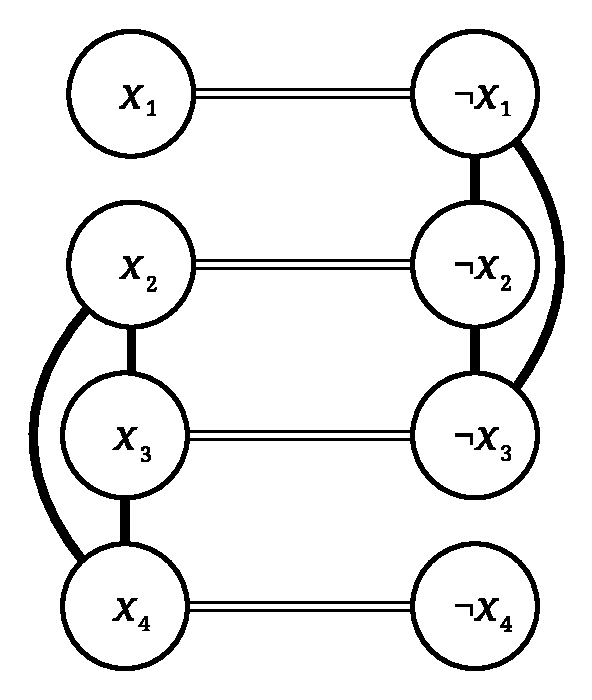
\includegraphics[width=4cm]{gconf.pdf}
\end{minipage}
\caption{Conflict graph for equations \ref{eq:1} and \ref{eq:2} }\label{graph}
\end{figure}





Figure \ref{graph} shows the conflict graph for this constraints, where $\neg x_i$ represents the complement (or deactivation) of variable $x_i$. Edges represent conflicts between variables or complimentary variables (double edges). For the constraint of equation \ref{eq:1}, we have to transform it in a $\leq$-constraint, multiplying by -1. So, we have: $- x_1 - x_2 - x_3 \leq - 2$. How the coefficients of this constraints are ordered, we can start calculating $L_{\ref{eq:1}}^{x_{\hat{j}}=1,\, x_{\hat{j}+1}=1}$. For any pair of activated variables we are able to produce a solution that respects this constraint. For this reason we do not find a clique with active variables in this constraint. Calculating $L_{\ref{eq:1}}^{x_{\hat{j}}=0,\, x_{\hat{j}+1}=0}$ for the first pair of subsequent variables (i.e. $\hat{j}=1$) we find a conflict that implies in a clique involving all complement of the variables starting from $x_1$ until $x_3$ ($L_{\ref{eq:1}}^{x_1=0,\, x_2=0} = -1$). So, we insert this conflicts in the graph.

We proceed analyzing the constraint of equation \ref{eq:2}. For any pair of deactivated variables we are able to produce a solution that respects this constraint. For this reason we do not find a clique with deactivated variables in this constraint. Calculating $L_{\ref{eq:2}}^{x_{\hat{j}}=1,\, x_{\hat{j}+1}=1}$ for the consecutive pairs of variables we can found a clique starting from $x_2$ until $x_4$ ($L_{\ref{eq:2}}^{x_{2}=1,\, x_{3}=1} = 5$). We finish inserting this conflicts in the graph.

\end{example}


\section{Cutting Planes}\label{cut}

Linear programming relaxations can be significantly strengthened by the inclusion of inequalities derived from the set packing polytope (SPP) \cite {Padberg1973}. The most common classes of cuts for SPP are the clique cuts and the odd-hole cuts. A clique inequality for a set $C$ of conflicting variables has the form $\sum_{j\in C}x_{j} \leq 1$ and an odd-hole inequality with conflicting variables $C$ can be defined as: $\sum_{j\in C}x_{j} \leq \lfloor \frac{|C|}{2}\rfloor$. It is well known that in practice clique cuts are by far the most important ones \cite{Borndorfer1998}. The impact of these cuts has been explored for some hard timetabling problems \cite{Avella2005,Marecek2012}. Considering generic clique separation routines, the most common ones are the star clique and the row clique method \cite{Eso1999a,Hoffman1993,Borndorfer1998}. These are fast separation routines which are used in the current version of the COIN-OR Cut Generation Library.  

Our algorithm proposal considers aggressive clique separation: instead of searching for \emph{the} most violated clique inequality we search for \emph{all} violated clique inequalities. Some previous results indicate that this is the best strategy. In \cite{Marecek2012}, for example, although authors used a branch-and-bound code to search for the most violated clique, computational results motivated the inclusion of non-optimally violated cuts found during the search. This result is consistent with reports of application of other cuts applied to different models, such as {C}hv\`{a}tal-Gomory cuts \cite{Fischetti2007}. The option for inserting a large number of violated inequalities at once is also responsible for reviving the gomory cuts importance \cite {Cornuejols2007}.

Our proposed clique separation routine has two main components:  \begin{enumerate} \item a module to separate all violated cliques in the conflict subgraph induced by the fractional variables; \item a lifting module which extends generated cliques considering the original conflict graph. \end{enumerate}  The clique separation module was implemented using an improved version of the Bron-Kerbosch algorithm \cite{Bron1973}. This version implements an optimized pivoting rule \cite{Brito2011} to speed up the discovery of maximal cliques with large weight. This rule assigns the highest priority for visiting first nodes with large modified degree (summation of node degree and of its neighbors) and weight. Although this algorithm has an exponential worst case performance, the heuristic pivot rules  make the algorithm suitable not only for running in the enumeration context but also for executing with restricted times, since larger violated cliques tend to be discovered first. Nevertheless, our experiments showed that all violated inequalities for all instances can be enumerated in a fraction of a second using our implementation. It is also important to remark that even if a subset of cliques is inserted, the optimal solution would not be missed, branching would take care of the rest.  The importance of lifting clique inequalities can be explained with the conflict graph in Figure \ref{figClique}. Nodes inside the gray area indicate variables with non-zero values in the fractional solution. In this solution, only nodes $x_{2},\ldots,x_{4}$ could contribute to define a maximally violated clique inequality. Nevertheless, subsequent linear programming relaxations could include three different violated $k_{3}$\footnote{a clique with three nodes} cliques by alternating the inactive variable. If the $k_{4}$ clique inequality were inserted during the separation of the first fractional solution, additional re-optimizations of the linear program could be saved. Furthermore, a less dense constraint matrix may be obtained with the insertion of these dominant constraints first.

\begin{figure}
\begin{center}
	\includegraphics[width=0.3\textwidth]{clique.pdf}
	\caption{Example of a $k_{3}$ which could be lifted to a $k_{4}$ } \label{figClique}
\end{center}
\end{figure}

It is well known that the separation of odd-holes contributes only marginally for lower bound improvement \cite{Borndorfer1998,Mendez-Diaz2008}. Nevertheless, its inclusion in the branch-and-cut procedure is cheap, since these inequalities can be separated in polynomial time using shortest path algorithms \cite{Grotschel1993}. Odd hole inequalities can be strengthened by the inclusion of a wheel center, such as variable $x_{6}$ in the conflict graph presented in Figure \ref{figOH}. In fact, for an odd hole with variables $C$ and $W$ being the set of candidates to be included as wheel centers of $C$, the following inequality is valid:

\begin{equation}
	\sum_{j \in W} \lfloor \frac{|C|}{2} \rfloor x_{j} + \sum_{j \in C} x_{j} \leq \lfloor \frac{|C|}{2} \rfloor
\end{equation}

\begin{figure}
\begin{center}
	\includegraphics[width=0.3\textwidth]{oddHole.pdf}
	\caption{Example of an odd hole and its possible extension to a wheel} \label{figOH}
\end{center}
\end{figure}


\section{Experimental Results}\label{experiments}
\section{Conclusions and Future Work}\label{conclusions}


%\begin{acknowledgements}
%If you'd like to thank anyone, place your comments here
%and remove the percent signs.
%\end{acknowledgements}

% BibTeX users please use one of
%\bibliographystyle{spbasic}      % basic style, author-year citations
\bibliographystyle{spmpsci}      % mathematics and physical sciences
%\bibliographystyle{spphys}       % APS-like style for physics
\bibliography{references}   % name your BibTeX data base

% Non-BibTeX users please use
% \begin{thebibliography}{}
%
% and use \bibitem to create references. Consult the Instructions
% for authors for reference list style.
%
% \bibitem{RefJ}
% Format for Journal Reference
% Author, Article title, Journal, Volume, page numbers (year)
% Format for books
% \bibitem{RefB}
% Author, Book title, page numbers. Publisher, place (year)
% etc
% \end{thebibliography}

\end{document}
% end of file template.tex

